\documentclass[letterpaper, 12pt]{article}
\usepackage{setspace} %espaciado
\usepackage{fontspec} %manejo de distintas tipografías
\usepackage[letterpaper, top=2.5cm, bottom=2.5cm, left=3cm, right=3cm]{geometry} %margenes
\usepackage[utf8]{inputenc} %manejo de caracteres especiales
\usepackage[spanish]{babel} %manejo de encabezados de inglés a español
\usepackage{fancyhdr} %formato de los encabezados de página
\usepackage{ragged2e} %alineado real justficado
\usepackage{graphicx} %manejo de imagenes
\usepackage{amsmath} %manejo de notación matemática
\usepackage{mathtools} %manejo de notación matemática
\usepackage{blindtext} %texto de relleno
\usepackage{amssymb} %manejo de simbología variada
\usepackage[backend=biber]{biblatex} \addbibresource{referencias.bib}%bibliografía 
\usepackage[titles]{tocloft} %manejo de elementos para el índice
\usepackage{float} %manejo de centrado para figuras
\usepackage{hyperref} %manejo d hipervínculos

%color de los hipervinculos
\hypersetup{
    colorlinks=true,      
    urlcolor=blue,
    linkcolor=blue
}

%formato de los encabezados y pies de página
\pagestyle{fancy}
\fancyhf{}
\rfoot{\thepage}

%permite la impresión de las referencias sin haberlas citado explicitamente en el documento
\nocite{*}

\renewcommand{\headrulewidth}{0pt} %eliminar la barra del encabezado

%fuente arial (COMPILAR DESDE LA CONSOLA CON xelatex)
\setmainfont{Arial}

%interlineado de 1.5
\setstretch{1.5}

\begin{document}
    
    %PORTADA
    \begin{titlepage}
        \begin{figure}[ht]
            \centering
            
\includegraphics[width=15cm]{logosITT.png}
        \end{figure}
        \centering
        {\scshape\LARGE Tecnológico Nacional de México\\Instituto Tecnológico de Tijuana\par}
        \vspace{1cm}
        {\scshape\Large Investigación de Operaciones\par}
        \vspace{1cm}
        {\scshape\Large Unidad 4\par}
        \vspace{1.5cm}
        {\huge\bfseries Teoría de Inventarios\par}
        \vspace{2cm}
        {\Large\itshape Chino Jimenez Kevin Alejandro,\, 19211616\\Flores Azcona Abraham Jhared,\,19211640\\Gonzales Guzman Maria Jose,\,19211650\\Sanchez Deseusa Victor Manuel,\,19211732\par}
        \vfill
        Profesora: \par
        Ing. Igreyne Aracely Ruiz Romero
        
        \vfill

        {\large 6 de diciembre del 2020}
    \end{titlepage}

    \newpage
    \thispagestyle{empty}
    \tableofcontents
    \listoffigures

    %CUERPO
    \newpage
    \lhead{\textbf{Unidad 4. Teoría de Inventarios}}
    \rhead{\textbf{Introducción}}
    \section*{Introducción}
    \addcontentsline{toc}{section}{Introducción}
    \justify
    En este documento se desarrollan los temas que componen a la 4ta. unidad de la materia de Investigación de Operaciones, los cuales revuelven
    en los inventarios  la teoría detrás de ellos; aparte se pretende dar a conocer las herramientas para mejorar la toma de desiciones sobre inventarios,
    ya que nos da elementos para la manipulación de estos.

    %glosario
    \newpage
    \lhead{\textbf{Unidad 4. Teoría de Inventarios}}
    \rhead{\textbf{Glosario}}
    \section*{Glosario}
    \addcontentsline{toc}{section}{Glosario}
    \justify    
    Como cualquier tema, es necesario tener en cuenta ciertos conceptos para mantener un mejor entendimiento en el trancurso del escrito. Consideramos que los expuestos en esta sección son los relevantes (se muestran por orden alfabético):
    \\\newline
    \textbf{Algorítmo:} Conjunto ordenado de operaciones sistemáticas que permiten obtener un resultado a un problema.
    \\
    \textbf{Almacén:} Local, edificio o parte de este que sirve para depositar o guardar gran cantidad de artículos, productos o mercancías para su posterior venta, uso o distribución.
    \\
    \textbf{Aritmética:} Parte de la matemática que estudia los números y las operaciones que se hacen con ellos.
    \\
    \textbf{Caóticos:} Que es absolutamente desordenado o confuso.
    \\
    \textbf{Déficit:} Cantidad que falta a los ingrsos para que se equilibren con los gastos.
    \\
    \textbf{Determinísta:} Que sigue la doctrina filosófica del determinismo o que es partidaria del determinismo. En el contexto de la unidad, nos referimos a que sea un dato finíto y que se pueda obtener.
    \\
    \textbf{FIFO:} Siglas de \emph{First In, First Out} (Primeras Entradas, Primeras Salidas). La valoración del inventario y el manejo en el almacén de los mismos se basa en costos más recientes.
    \\
    \textbf{Hipotéticas:} Que está basado en una hipótesis o en una suposición.
    \\
    \textbf{LIFO:} Siglas de \emph{Last In, First Out} (Ultimas Entradas, Primeras Salidas). La valoración del inventario y su manejo en el almacén se basa en costos estables cuando ocurre algún alza en los precios.
    \\
    \textbf{Linearización:} En las ramas de las matemáticas se refiere a encontrar aproximaciones lineales a funciones en un punto dado. Permite estudiar la estabilidad local de un punto de equilibrio de un sistema de ecuaciones diferencales no lineales.
     
    \newpage
    \lhead{\textbf{Unidad 4. Teoría de Inventarios}}
    \rhead{\textbf{Marco Teórico}}
    \section*{Marco Teórico}
    \addcontentsline{toc}{section}{Marco Teórico}
    \justify
    La Teoría de Inventarios procura alcanzar un equilibrio sobre las cantidades que se desean pedir y los tiempos exactos para pedirlos; a su vez considerando los costos
    pensando el el beneficio de la empresa. Esto nace (junto a la propiedad privada) por la necesidad de organizar los bienes que se poseen en el momento y mantener un control 
    sobre los mismos. El pasar de los años ha dado la evolución de los manejos de inventarios y por esto es relevante mantenerse a la vanguardia de algo tán mundano pero tan relevante para
    los negocios y la cotidianeidad.
    \subsection*{Inventario}
    \justify
    El inventario representa la existencia de bienes almacenados destinados a realizar una operación, sea de compra, venta, alquiler, uso o tranformación. Debe aparecer (en términos de contabilidad) dentro de las cuentas de activo
    como \emph{activo circulante}. Esto es debido a que la naturaleza del activo circulante clasifica todas las cuentas las cuales su costo siempre es variable.
    \\\newline
    A grandes rasgos, un inventario puede ser algo tan cotidiano como un guardarropa de atuendos, o algo tán elaborado como las distintas partes de un proceso de manufactura. Esto nos lleva a que los inventarios de las compañias pueden variar
    bastante según el giro de la empresa y por ende, lo que necesitan para realizar sus deberes.
    \subsection*{Tipos de inventario}
    \justify
    A continuación, se enlistan los distintos tipos de inventario generalmente empleados en distintas compañias de manufactura:
    \begin{itemize}
        \item \emph{Materias primas:} Lo conforman aquellos materiales no procesados que se requiern para elaborar los productos.
        \item \emph{Productos en proceso de fabricación:} Lo integran aquellos bienes adquiridos los cuales están en el proceso de manufactura.
        \item \emph{Productos terminados:} Lo conforman aquellos bienes los cuale ya están listos para ser vendidos como productos de la empresa.
    \end{itemize}
    \subsection*{Valuación de inventarios}
    \justify
    Contablemente, son las maneras en las cuales podemos obtener el verdadeo costo de nuestro inventario. Dependiendo de la situación del mercado y las necesidades de la empresa, se aplica la valuación respectiva. Los más relevantes y los más sencillos
    de comprender son los siguientes:
    \begin{itemize}
        \item \emph{FIFO (First In, First Out):} Conocido en español como \emph{Primeras Entradas, Primeras Salidas}. Su valoración se adapta más a la realidad del mercado, ya que emplea dicha valuación con los costos más recientes.
        \item \emph{LIFO (Last In, First Out):} Conocido en español como \emph{Ultimas Entradas, Primeras Salidas}. Su valoración se mantiene estable si ocurre un alza de precios.
        \item \emph{Costo Promedio Aritmético: } Como su nombre lo indica el resultado de valoración se dará por la media aritmética de los precios unitarios de los articulos.
    \end{itemize}
    
    \newpage
    \lhead{\textbf{Unidad 4. Teoría de Inventarios}}
    \rhead{\textbf{Sistemas de administración y control}}
    \section{Sistemas de administración y control}
    \justify
    Uno de los principales puntos a elaborar son los sistemas de administración y control. Para un buen control de inventarios es necesario tener un buen sistema de este tipo. Una organización necesita especificar un sistema a controlar y planear las distintas operaciones
    que maneja. Las cuatro razones por la necesidad de los sistemas de administración y control son los siguientes:
    \begin{itemize}
        \item Toda organización tiene objetivos organizacionales definidos.
        \item La administración tiene una jerarquía, con sub-unidades de administradores. Cada administrador tiene que definir sus objetivos personales, los cuales deben de alinearse con los objetivos de la organización.
        \item Situaciones organizacionales, junto al comportamiento humano, crean una situación de incertidumbre y dicha incertidumbre está presente en circunstancias internas y externas.
        \item Los objetivos deben ser optimizados y el esfuerzo humano debe ser una variable en esos objetivos.
    \end{itemize}
    En términos más concretos, los SAC (Sistemas de administración y control) aseguran que la planeación estratégica y el control de operaciones puedan realizarze, porque los SAC aseguran que los recursos son obtenidos y empleados efectiva y eficientemente en el cumplimiento de los objetivos
    de la organización en cuestión.
    \\\newline
    La primer caraterística de ellos es la estructura y la subsecuente hace referencia a los proceso que maneja. Se puede considerar de la siguiente manera:
    \begin{itemize}
        \item \emph{El diseño del sistema es acerca de la estructura del SAC.}
        \item \emph{El rendimiento del sistema es un indicador del proceso del SAC.}
    \end{itemize}
    Los beneficios de aplicar dichos sistemas son varios. El principal es reducir los riesgos debido a que el ente asegura un rendimiento actual y los resultados referentes a los objetivos principales de la organización por los SAC que le brindan movimiento hacia los mismos. Permite observar loss problemas con mayor detalle
    porque la estructura jerarquía es definida y, por ende, si una de las partes no cumple su labor, afecta las demás. También permite mejorar la planeación a largo plazo por dicha claridad y apego a los SAC. En otras palabras, define lo siguiente:
    \begin{itemize}
        \item \textbf{El tamaño, el alcanze y la estructura de la organización.}
        \item \textbf{La naturaleza de las operaciones y su divisibilidad.}
        \item \textbf{La variedad de las responsabilidades dentro de la organización.}
        \item \textbf{Las personas de la organización y sus percepciones de la misma.}
    \end{itemize}
    Su aplicación dentro de la Teoría de los Inventarios permite un mayor rendimiento de los recursos y una mejor transparencia con el manejo de los mismos. Una gran alegoría son los engranajes de una máquina, si uno de ellos se atasca, dicha máquina deja de funcionar acorde a lo esperado.
    \begin{figure}[H]
        \centering
        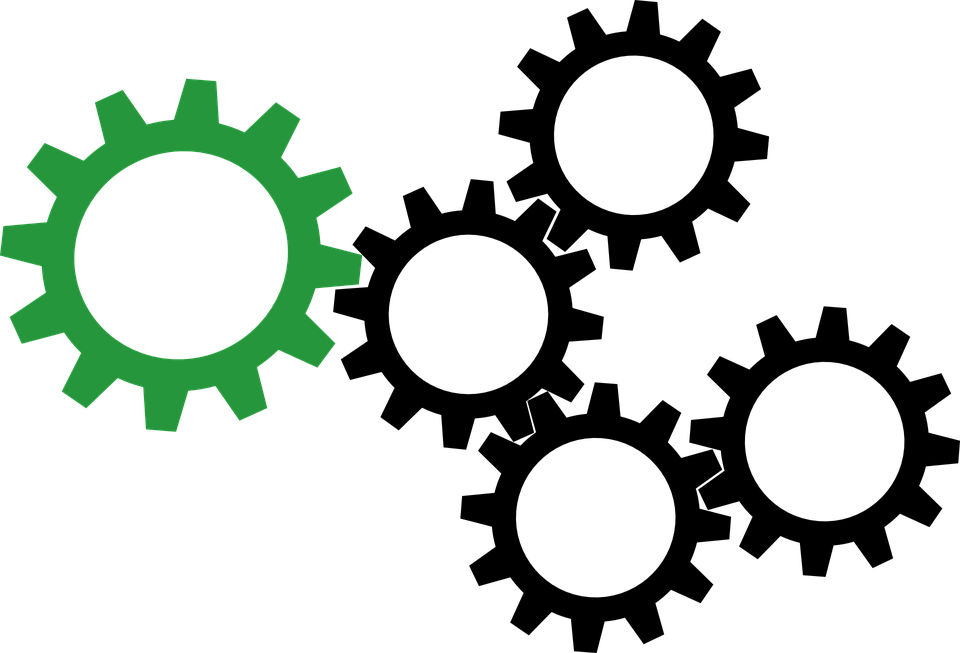
\includegraphics[width=10cm]{gears.png}
        \caption{Engranajes. }
    \end{figure}

    \newpage
    \lhead{\textbf{Unidad 4. Teoría de Inventarios}}
    \rhead{\textbf{Modelos determinísticos}}
    \section{Modelos determinísticos}
    \justify
    Un modelo determinísta es un modelo matemático donde las mismas entradas o condiciones iniciales producirán invariablemente las mismas salidas, no contemplándose la existencia de azar, o incertidumbre en el proceso mediante dicho modelo.
    \\\newline
    Está estrechamente relacionado con la creación de entornos simulados a través de simuladores para el estudio de situaciones hipotéticas, o para crear sistemas de gestión que peermitan disminuir la propagación de errores. Los modelos deterministas sólo pueden
    ser adecuados para sistemas deterministas no caóticos, para sistemas azarosos y caóticos.
    \\\newline
    Un conjunto de ecuaciones diferenciales de un sistema físico macroscópico constituye un modelo determinista que puede predecir la evolución determinista en el tiempo de un buen número de magnitudes características del sistema. 
    \\\newline
    Los modelos determinísticos son relevantes debido a que:
    \begin{itemize}
        \item Existe una gran variedad de problemas importantes de administración que pueden formularse como modelos determinísticos.
        \item Muchas hojas de cálculo electrónicas cuentan con la tecnología necesaria para opimizar modelos determinísticos, es decir, para encontrar desiciones óptimas. Cuando se trata de modelos de Programación Lineal grandes, el procedimiento puede realizarse con mucha rapidez y fiabilidad.
        \item El subproducto de las técnicas de análisis es una gran cantidad de información extremadamente útil para la interpretación de los resultados por la administración.
        \item La optimización restringida, en particular, es un recurso extremadamente útil para reflexionar acerca de situaciones concretas, aunque no piense usted construir un modelo para optimizarlo.
        \item La práctica con modelos determinísticos ayuda a desarrollar habilidad para formular modelos.
    \end{itemize}
    \subsection{Lotes económicos sin déficit}
    \justify
    En el Lote económico sin déficit el inventario se puede reabastecer cuando el nivel baje lo suficiente, pero para ello se supondrá primero que no se admitn faltantes, con la tasa de demanda fija, se puede evitar los faltantes al reabastecer
    el inventario cada vez que el nivel baje a cero.
    \\\newline
    El objetivo consiste en determinar con qué frecuencia y en qué cantidad se debe reabastecer el inventario de manera que se minimíce la suma de estos costos por unidad de tiempos.
    \\\newline
    Dentro de los distintos de modelos de inventarios, el modelo más apropiado para tener una noción del tema es del EOQ, que traducido al español es el \emph{Modelo de Orden Económico Cuantitativo sin faltante}. Dicho modelo es uno determinístico que
    se caracteriza por lo siguiente:
    \begin{itemize}
        \item La demanda es constante y conocida.
        \item No admite faltante.
        \item Existe un costo de mantenimiento del inventario.
        \item Existe un costo por pedir.
        \item Los costos siempre son constantes.
        \item En la reposición no existe un tiempo en de demora en los pedidos. Estos siempre llegan completos.
    \end{itemize}
    Para trabajar este modelo es necesario una gráfica referente a la cantidad de articulos del inventario con respecto al tiempo.
    \begin{figure}[H]
        \centering
        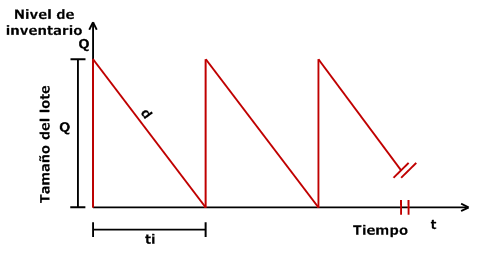
\includegraphics[width=10cm]{graficaeoq.png}
        \caption{Gráfica representativa del modelo EOQ sin faltante}
    \end{figure}
    \justify
    Con la información de la gráfica anterior es posible obtener la ecuación para el costo del tamaño del lote en un periodo dado:
    \[C(Q)=C_uQ+C_p+C_{mi}\left(\frac{t_iQ}{2}\right)\]
    \justify
    Donde:
    \begin{itemize}
        \item \(C(Q)\,\): Costo en un periodo en función de \(Q\).
        \item \(C_u\,\): Costo de adquisición.
        \item \(C_p\,\): Costo de pedido.
        \item \(C_{mi}\,\): Costo del mantenimiento del inventario.
        \item \(t_i\,\): Tiempo en el periodo \(i\).
    \end{itemize}
    A grandes rasgos, es la ecuación de lote económico \(Q\) para el modelo de costo de faltantes debido a las ventas perdidas aumentan hasta cierto valor, el radical que determina \(Q\) se vuelve negativo.
    Esto indica el costo por faltantes por conceptos de ventas perdidas cuando estas son muy grandes, el cual no es conveniente para trabajar con la políitica de pedidos pendientes.
    \\\newline
    \[\text{CTO}=\frac{DC_o}{Q}\]
    \[\text{CTM}=\frac{QC_m}{2}\]
    \[\begin{matrix}
        \text{CTO}&=&\text{CTM}\\
        \frac{DC_o}{Q}&=&\frac{QC_m}{2}\\
        2DC_o&=&Q^2C_m\\
        Q^2&=&\frac{DC_0}{C_m}\\
        Q&=&\sqrt{\frac{DC_0}{C_m}}
    \end{matrix}\]
    Donde:
    \begin{itemize}
        \item \(CTO\): Costo total por ordenar.
        \item \(CTM\): Costo total de mantenimiento.
        \item \(Q\): Cantidad óptima a pedir.
        \item \(C_o\): Costo por ordenar el pedido.
        \item \(D\): Demanda por unidad de tiempo
    \end{itemize}
    \subsection{Lotes económicos con déficit}
    \justify
    Lo contrario al modelo anterior, ahora se trabaja con escasez de productos. Este modelo determina la cantidad a producir, cuando se permite déficit, faltantes o pedidos pendientes. Cabe destaca que un déficit (en términos financieros)
    es la cantidad faltante a los ingresos para equilibrar los gastos, dicho de otra manera, es el resultado negativo de la diferencia entre los ingresos y los gastos dle ente.
    \\\newline 
    Se supone que se inicia el inventario en cero unidades, que se coloca una orden de producción en ese instante u que dicha orden se completa en \(t_1\) unidades de tiempo; al final de éste se produce a razón de \(k\) unidades por unidad de tiempo y es consumido
    a razón de \(r\) unidades por unidad de tiempo. Existen en inventario \(S\) unidades. \\\newline
    Cuando se llega al inventario máximo, la producción se suspende y durante un tiempo de \(t_2\) unidades solo se suple la demanda, por lo tanto al final de este tiempo se encuentra en el nivel cero del inventario. A partir de aquí el cliente causa demanda, la cual no es satisfecha;
    esto sucede en \(t_3\) unidades de tiempo, al final se acumula una deuda de unidades con el cliente; déficit máximo.
    \\\newline
    Para satisfacerla, se coloca una nueva orden de producción con la cual se empieza a reducit el déficit y a cubrir la demanda de este tiempo \(t_4\), al final el tiempo se vuelve a repetir ya que la información es determinística y genera los ciclos.
    Para que dicho modelo funcione se requiere de lo siguiente:
    \begin{itemize}
        \item Tasa de producción con tasa constante.
        \item Tasa de producción mayor que tasa de demanda.
        \item Los costos deben deben ser conocidos y constantes.
    \end{itemize}
    A continuación, se muestra una gráfica representativa de dicho modelo:
    \begin{figure}[H]
        \centering
        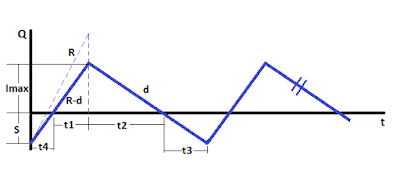
\includegraphics[width=10cm]{graficadeficit.png}
        \caption{Gráfica representativa del lote económico con déficit.}
    \end{figure}
    Donde:
    \begin{itemize}
        \item \(T\): Tiempo total del periodo de planeación.
        \item \(R\): Demanda total del periodo.
        \item \(r\): Tasa de demanda por unidad de tiempo.
        \item \(K\): Tasa de producción por unidad de tiempo.
        \item \(C_o\): Costo por ordenar una tanda de producción.
        \item \(S\): Nivel máximo de inventario.
        \item \(t_1\): Tiempo de producción y demanda hasta generar el superávit.
        \item \(t_2\): Tiempo de demanda hasta consumir el superávit.
        \item \(C_m\): Costo unitario de mantenimiento por unidad de tiempo.
        \item \(D\): Déficit máximo.
        \item \(t_3\): Tiempo de demanda hasta generar el déficit.
        \item \(t_4\): Tiempo de producción y demanda hasta cubrir el déficit.
        \item \(T_e\): Tiempo total del cíclo.
        \item \(C_p\): Costo unitario de penalización por unidad de tiempo.
        \item \(C_v\): Costo variable por unidad.
        \item \(C_t\): Costo total promedio por unidad de tiempo.
        \item \(C_T\): Costo total por unidad de tiempo.
        \item \(N\): Número de ciclos en el periodo.
        \item UMC: Unidades mantenidas por ciclo.
        \item \(C_{me}\): Costo de mantenimiento por ciclo.
        \item UPC: Unidades penalizadas por ciclo.
        \item \(C_{pe}\): Costo de penalización por ciclo.
    \end{itemize}
    \newpage
    \lhead{\textbf{Unidad 4. Teoría de Inventarios}}
    \rhead{\textbf{Lote económico de producción}}
    \section{Lote económico de producción}
    \justify
    El lote económico económico de producción (conocdio por sus siglas en inglés como \emph{Economic Production Quantity} ó \emph{EPQ}) es un modelo matemático para el control de inventarios que se extiende del modelo \emph{EOQ} (ó conocido como el modelo económico
    sin déficit). El principio fundamental de este modelo es encontrar el lote de producción de un único producto para el cual los costos por emitir la orden de producción y los costos por mantenerlo en el inventario se igualan.
    \\\newline
    Normalmente una orden de pedido es seguida de una orden de producción del artículo pedido, por lo que es necesario un cierto periodo de tiempo para completar dicha orden de producción. Durante este tiempo el artículo está siendo producido y demandado. Para que este caso tenga sentido
    la tasa de producción, tiene que ser mayor que la tasa de demanda, ya que si no fuese así no existiría inventario en ningun momento.
    \\\newline
    La empresa puede producir \(R\) unidades por unidad de tiempo. En cualquier instante la cantidad producida es \(Rt\). A continuación se muestra la sig. gráfica representativa:
    \begin{figure}
        \centering
        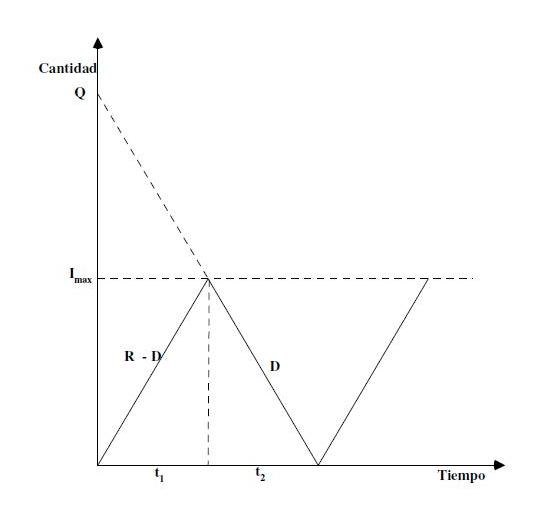
\includegraphics[width=10cm]{LED.JPG}
        \caption{Gráfica representativa del lote económico de producción.}
    \end{figure}
    La formula principal para este modelo es la siguiente:
    \[I=\frac{Q}{P}(P-D)=Q(1-\frac{D}{P})\]
    Donde:
    \begin{itemize}
        \item \(P\): Tasa de producción.
        \item \(Q\): Producción de la orden de pedido del lote.
        \item \(\frac{Q}{P}\): Tiempo de producción.
        \item \(P-D\): Tasa de acumulación del inventario.
        \item \(I\): Nivel máximo de inventario.
    \end{itemize}
    Otras formulas relevantes al modelo son las siguientes:
    \[\text{Costo anual de emisión: }\frac{D}{Q}\cdot C_E\]
    \[\text{Inventario Promedio: }\frac{Q}{2}\left(1-\frac{D}{P}\right)\]
    \[\text{Costo anual de mantenimiento de inventarios: }\frac{Q}{2}\left(1-\frac{D}{Q}\right)rc\]
    \[\text{Costo total anual: }\frac{D}{Q}\cdot C_E+\frac{Q}{2}\left(1-\frac{D}{Q}\right)rc\]
    \[\text{Lote óptimo: }Q=\sqrt{\frac{2DC_E}{rc\left(1-\frac{D}{P}\right)}}\]
    \newpage
    \lhead{\textbf{Unidad 4. Teoría de Inventarios}}
    \rhead{\textbf{Conclusión}}
    \section*{Conclusión}
    \addcontentsline{toc}{section}{Conclusión}
    \justify
    Esta sección se separan las conclusiones en las que correspoden a cada integrante y la que corresponde a nosotros como equipo. 
    \subsection*{Individual}
    \justify
    \textbf{Chino Jimenez Kevin Alejandro: }
    \\
    En la teoría de inventario se habla del inventario que tiene una empresa apra llevar un control de los bienes que tiene, y que cada empresa u organización tiene su propio inventario dependiente de los productos o servicios que se especializa.
    \\\newline
    Es de gran utilidad el tener conocimientos de este ya que hay métodos para que se sepa cuándo y cuántos del producto se tiene que invertir para que no sea afectada la empresa, y también para que no se llene el inventario limitado de la empresa.
    \\\newline
    \textbf{Flores Azcona Abraham Jhared: }
    \\
    Explorar de otra perspectiva el tema (a primera instancia) simple y sencillo como la Teoria de Inventarios permite plantear de una manera más matemática dicho tema, que aplicamos en la vida cotidiana. El complementar mis conocimientos adquiridos por las materias de Estructura de Datos y Contabilidad permitió bastante hilar a gran escala el tema expuesto. 
    \\\newline
    \textbf{Gonzales Guzman Maria Jose: }
    \\
    En síntesis se puede decir que la teoría de inventarios aporta una variedad de herramientas para poder llevar un control del inventario que posee determinada empresa o negocio principalmente de bienes.\\
    Las empresas requieren llevar un conteo y movimiento de su inventario además de estrategias para manejar la mercancía que tiene guardad para satisfacer las futuras demandas, sin que esta genere pérdidas o costos mayores, por lo tanto es de gran ayuda
    llevar a cabo los métodos vistos en la teoría de inventarios.
    \\
    \textbf{Sanchez Deseusa Victor Manuel: }
    \\
    El inventario se refiere a cualquier grupo de elementos destinados a realizar alguna operación, existen diferentes tipos de inventarios, materia prima, productos en proceso de fabricación; estos deben ser evaluados por alguno de los métodos existentes.
    \\\newline
    La importancia de llevar un control de inventario, recae en la necesidad de conocer la cantidad, el estado y la calidad de los productos, para realizar esto, es que existen los sistemas de administración y control, esto sirve para controlar las operaciones que se realizan sobre los elementos, conocer su mejor uso, la forma más eficáz y menos costosa de usarlos.
    \\\newline
    Lo interesante del inventario, es que cualquier cosa puede ser manejada como tal, desde un cuaderno con apuntes hasta un grupo de canicas en una caja, y aunque no tengamos un control escrito sobre ello, la verdad es que a veces lo hacemos de forma inconsciente y podemos entender como es el inventario en alguna empresa.
    \subsection*{General}
    \justify
    El estudio de la Teoría de Inventarios permite tanto a las empresas como a los individuos que colaboran en ellas el manejo optimizado y responsable de sus recursos para mantener una mejor gestión empresarial y sobre todo, más ganancias para los involucrados.
    %anexo
    \newpage
    \thispagestyle{fancy}
    \lhead{}
    \rhead{} 
    \section*{Anexo}
    \addcontentsline{toc}{section}{Anexo}
    \justify
    Siempre es recomendable tener control de cualquier cantidad de bienes materiales a disposición de cualquier entidad, compañia o institución, como también
    en nuestro hogar, permitiendo una mejor organización, sobre todo cuando es necesario realizar una mudanza o movilidad de un punto a otro dentro del hogar,
    así evitando perder material o bién llevando un mejor control de lo transportado.
    \\\newline
    Las funciones de un inventario añaden una flexibilidad operacional que no pudiese existir de otras maneras. En la manufactura, los inventarios de producto son
    necesidad importante, a menos que cada parte individual se lleve de máquina a máquina u que las mismas se preparen para producir un solo elemento. Dichas funciones son:
    \begin{itemize}
        \item Eliminación de irregularidades de la oferta.
        \item Compra o producción en lotes o tandas.
        \item Permitir a la organización el manejo de materiales perecederos.
        \item Almacenar la mano de obra.
    \end{itemize}
    \\\newline
    El mantener un buen estado del almacén también agiliza los inventarios que se realizen, debido a que ya se tendrá a la mano cada elemento previamente inventariado. 
    \begin{figure}[H]
        \centering
        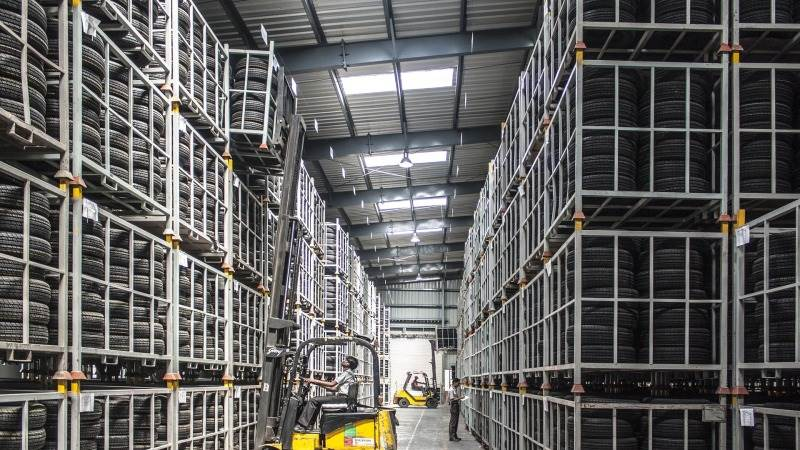
\includegraphics[width=10cm]{almacen.jpg}
        \caption{Ejemplo de un almacén.}
    \end{figure}
    %referencias
        %bibliografía
    \newpage
    \thispagestyle{fancy}
    \lhead{}
    \rhead{} 
    \begin{refsection}[referencias1.bib]
        \nocite{*}
        \printbibliography[title={Bibliografía}]
    \end{refsection}
    \addcontentsline{toc}{section}{Bibliografía}
        
        %páginas web
    \newpage
    \thispagestyle{fancy}
    \lhead{}
    \rhead{} 
    \printbibliography[title={Páginas web}]
    \addcontentsline{toc}{section}{Páginas web}

\end{document}